\documentclass[conference]{IEEEtran}
\usepackage[T1]{fontenc}
\usepackage{graphicx,booktabs,xcolor,url,listings,textcomp}
\usepackage{cite}
% AUTO-GENERATED by scripts/make_paper_artifacts.py. Do not edit.
\newcommand{\valMapFifty}{0.995}
\newcommand{\valMapFiftyNinetyFive}{0.934}
\newcommand{\valTrainMinutes}{32}
\newcommand{\valTrainEpochs}{15}
\newcommand{\valDefPrec}{75.9}
\newcommand{\valDefRec}{94.7}
\newcommand{\valDefEndToEnd}{92.1}
\newcommand{\valDefConf}{0.25}
\newcommand{\valDefFields}{374}
\newcommand{\valDefSeconds}{36}
\newcommand{\valDefEndToEndLo}{88.0}
\newcommand{\valDefEndToEndHi}{94.9}
\newcommand{\valDefOcrStage}{98.7}
\newcommand{\valFreePrec}{88.8}
\newcommand{\valFreeRec}{87.0}
\newcommand{\valFreeEndToEnd}{84.6}
\newcommand{\valFreeConf}{0.45}
\newcommand{\valFreeFields}{294}
\newcommand{\valFreeSeconds}{31}
\newcommand{\valFreeEndToEndLo}{79.5}
\newcommand{\valFreeEndToEndHi}{88.6}
\newcommand{\valFreeOcrStage}{100.0}
\newcommand{\valNmsPrec}{98.7}
\newcommand{\valNmsRec}{99.3}
\newcommand{\valNmsEndToEnd}{97.1}
\newcommand{\valNmsConf}{0.15}
\newcommand{\valNmsFields}{302}
\newcommand{\valNmsSeconds}{30}
\newcommand{\valNmsEndToEndLo}{94.1}
\newcommand{\valNmsEndToEndHi}{98.6}
\newcommand{\valNmsOcrStage}{97.9}
\newcommand{\valNmsChosenValF}{99.0}
\newcommand{\valFreeChosenValF}{88.4}
\newcommand{\valBaseCapture}{99.6}
\newcommand{\valBaseLo}{97.7}
\newcommand{\valBaseHi}{99.9}
\newcommand{\valBaseSecPerDoc}{0.63}
\newcommand{\valDefDup}{90}
\newcommand{\valDefMissed}{16}
\newcommand{\valDefDupConf}{0.59}
\newcommand{\valDefTopConf}{0.72}
\newcommand{\valNmsOcrErrCount}{5}
\newcommand{\valNmsOcrErrAllAccount}{all}
\newcommand{\valOcrErrExamples}{\texttt{8302653675} read as \texttt{B302653675}; \texttt{4077916523} read as \texttt{1077916523}; \texttt{0188416938} read as \texttt{018841693}}
\newcommand{\valPrecAccountNumber}{100.0}
\newcommand{\valRecAccountNumber}{96.7}
\newcommand{\valOcrAccountNumber}{91.4}
\newcommand{\valPrecDate}{100.0}
\newcommand{\valRecDate}{100.0}
\newcommand{\valOcrDate}{100.0}
\newcommand{\valPrecAmount}{100.0}
\newcommand{\valRecAmount}{100.0}
\newcommand{\valOcrAmount}{100.0}
\newcommand{\valPrecName}{93.8}
\newcommand{\valRecName}{100.0}
\newcommand{\valOcrName}{100.0}
\newcommand{\valPrecSignature}{100.0}
\newcommand{\valRecSignature}{100.0}
\newcommand{\valOcrSignature}{n/a}
\newcommand{\valPatDocs}{48}
\newcommand{\valPatParts}{2}
\newcommand{\valPatRepeats}{3}
\newcommand{\valPatRowUdfSec}{9.4}
\newcommand{\valPatRowUdfSd}{0.4}
\newcommand{\valPatRowUdfDps}{5.1}
\newcommand{\valPatRowUdfSpeedup}{1.0}
\newcommand{\valPatPartOneSec}{5.7}
\newcommand{\valPatPartOneSd}{0.1}
\newcommand{\valPatPartOneDps}{8.5}
\newcommand{\valPatPartOneSpeedup}{1.7}
\newcommand{\valPatPartSixteenSec}{5.6}
\newcommand{\valPatPartSixteenSd}{0.1}
\newcommand{\valPatPartSixteenDps}{8.6}
\newcommand{\valPatPartSixteenSpeedup}{1.7}
\newcommand{\valPatBoxes}{300}
\newcommand{\valPatLoadMs}{167}

\urldef{\repourl}\url{https://github.com/REPLACE-WITH-YOUR-ACCOUNT/findoc-yolo26-spark}
\lstset{basicstyle=\ttfamily\scriptsize,breaklines=true,frame=single,xleftmargin=2pt,xrightmargin=2pt,
  keywordstyle=\color{blue!60!black},commentstyle=\color{gray},showstringspaces=false,captionpos=b,aboveskip=4pt}
\makeatletter
\renewcommand\IEEEkeywordsname{Index Terms}
\def\abstract{\normalfont\bfseries\itshape Abstract. \bfseries}
\def\IEEEkeywords{\normalfont\bfseries\itshape Index Terms. \bfseries}
\makeatother
\begin{document}
\title{Field-Level Financial Document Extraction with YOLO26 and Apache Spark: A Reproducible Pipeline, Its Failure Modes, and a Controlled Evaluation}
\author{\IEEEauthorblockN{Ram Ghadiyaram}\IEEEauthorblockA{Independent Researcher\\Celina, TX, USA\\ram.ghadiyaram@gmail.com\\ORCID: 0009-0006-3730-0914}
\and\IEEEauthorblockN{Sashi Kiran Kaata}\IEEEauthorblockA{Independent Researcher\\Glendale, AZ, USA\\sashikiran9@gmail.com\\ORCID: 0009-0002-7980-2905}}
\maketitle
\begin{abstract}
Putting a vision model inside a Spark job looks routine and fails quietly. We build a field-level document extraction pipeline in which YOLO26 localizes fields and Tesseract reads each crop, executed with \texttt{mapInPandas} so the model loads once per partition. We catalog the integration defects that made a first version wrong, each checked against a running system, including a Spark image source that returns decoded pixels instead of file bytes and an Arrow failure on Spark 3.5 with JDK 21. On a synthetic form dataset with exact ground truth, a CPU-fine-tuned YOLO26n reaches \valNmsPrec\% detection precision and \valNmsRec\% recall, and \valNmsEndToEnd\% of text fields are read correctly end to end. Without class-wise suppression the end-to-end head emitted \valDefDup{} duplicate boxes and precision fell to \valDefPrec\%. Full-page Tesseract captured \valBaseCapture\% of the strings but does not say which field they belong to, so we do not claim an accuracy advantage. Loading the model per partition was \valPatPartSixteenSpeedup{} times faster than per row on two CPU cores. Data are synthetic and no GPU, EMR, or Textract measurements are reported. All numbers are generated from files in the released repository.
\end{abstract}
\begin{IEEEkeywords}
Financial document intelligence, YOLO26, Apache Spark, document field extraction, OCR, reproducibility.
\end{IEEEkeywords}
\section{Introduction}
Financial institutions ingest checks, identification forms, and statements as images, and downstream systems need to know which string is the account number, which is the date, and which is the amount. Page-level OCR returns text but not that mapping, and its accuracy is not a fixed number: published evaluations report Tesseract anywhere from 47 percent accuracy on Thai vehicle registration certificates \cite{thammarak2022} to 92.6 percent word recognition on letters \cite{reisswig2019}, with different metrics, document types, resolutions, and preprocessing. A detect-then-read design addresses both problems. An object detector localizes each field, and OCR runs only on the cropped region, so every extracted string arrives already labeled with its field class.

Ultralytics YOLO26 \cite{jocher2026yolo26} is a natural detector for this role. Its end-to-end head does not need non-maximum suppression at inference, which removes a post-processing pass from the serving path. Running it over millions of documents calls for a distributed engine, and Apache Spark \cite{zaharia2012} is the usual choice.

The difficulty is that a model call inside a Spark job looks routine and fails quietly. The RAPIDS Accelerator for Apache Spark \cite{nvidia_udf,nvidia_rapids} accelerates Spark\textquotesingle{}s own SQL and DataFrame plan on GPU. It does not accelerate Python code that loads a model inside a user-defined function, so enabling it does not make model inference fast. The first version of this pipeline contained several such defects, some in the model call pattern, some in data access, and some in the toolchain. We found them only after running the code, which is the reason this paper reports a running system and not a design alone.

This paper builds the pipeline, runs it, measures it, and releases it. Its scope is deliberately narrow. All reported accuracy is on a synthetic form dataset whose labels are exact by construction, timing is on a two-core CPU with one replication on a single GPU, and the AWS EMR and multi-GPU deployment is presented as design, not as measurement.

\section{Contributions}
\begin{itemize}
\item A complete open implementation of field detection, field-level OCR, and aggregation as one Spark job, with unit and end-to-end tests. One command reproduces the CPU results, and a notebook repeats the study on a GPU.
\item A catalog of integration defects, marked by whether we reproduced them by running code or found them by inspection, and the corrected partition-level inference pattern that resolves them (Section~\ref{sec:impl}).
\item An evaluation on a dataset with exact ground truth, with one training run per device: detection precision and recall, end-to-end field accuracy against a full-page Tesseract baseline, and a measured comparison of three ways to run the same model inside Spark (Section~\ref{sec:results}).
\item A deployment design for AWS EMR with RAPIDS, kept separate from what was measured, including when the batch design is and is not appropriate (Section~\ref{sec:design}).
\end{itemize}

\section{Related Work}
\textbf{Detection.} Single-network detection was introduced by Redmon et al.\ \cite{redmon2016}. YOLOv9 added programmable gradient information \cite{wang2024yolov9}, and YOLOv10 was the first in the line to remove non-maximum suppression \cite{wang2024yolov10}. YOLO26 keeps native end-to-end inference, removes Distribution Focal Loss, and is a recent Ultralytics release \cite{jocher2026yolo26}. DocLayout-YOLO adapts the family to document layout analysis \cite{zhao2024doclayout}. We use YOLO26 because it is the maintained production model and its NMS-free head simplifies the serving path. We do not claim it is the best detector for financial fields, and we do not compare against other detectors.

\textbf{OCR and document understanding.} Tesseract \cite{smith2007} remains a common open-source engine, and its accuracy varies widely with document type and preprocessing \cite{thammarak2022,reisswig2019}. Managed services such as Amazon Textract \cite{textract} are an obvious comparison, which we do not make because it needs an AWS account and real documents. Layout-aware transformers such as LayoutLMv3 \cite{huang2022layoutlmv3} and OCR-free models such as Donut \cite{kim2022donut} are stronger, heavier alternatives that solve a broader problem. Our baseline is Tesseract alone, which makes the comparison one of pipeline structure, not one against the state of the art.

\textbf{Datasets.} FUNSD \cite{jaume2019} and SROIE \cite{huang2019sroie} are the public datasets closest to this domain, and neither fits. FUNSD annotates form entities as question, answer, header, and other. SROIE provides text-line boxes and key-information strings for receipts. Neither provides region boxes for classes such as account number, date, amount, name, and signature. For that reason we evaluate on a synthetic dataset whose boxes and strings are exact, and we say plainly what that does and does not show.

\textbf{Systems.} Spark\textquotesingle{}s resilient distributed datasets \cite{zaharia2012} underlie its DataFrame engine. Spark exchanges data with Python through Apache Arrow, and \texttt{mapInPandas} \cite{spark_mapinpandas} exposes that path at partition granularity. Spark can schedule GPUs as task resources \cite{spark_resources}, and the RAPIDS documentation describes how GPU-scheduled Python workers share a device with the executor \cite{nvidia_udf}.

\section{System Design}\label{sec:design}
Fig.~\ref{fig:arch} shows the full ingestion-to-analytics design. Solid boxes inside the Spark job are implemented and measured in this paper. Dashed boxes are the AWS deployment around it, which we describe but did not run.

\begin{figure*}[t]
\centering
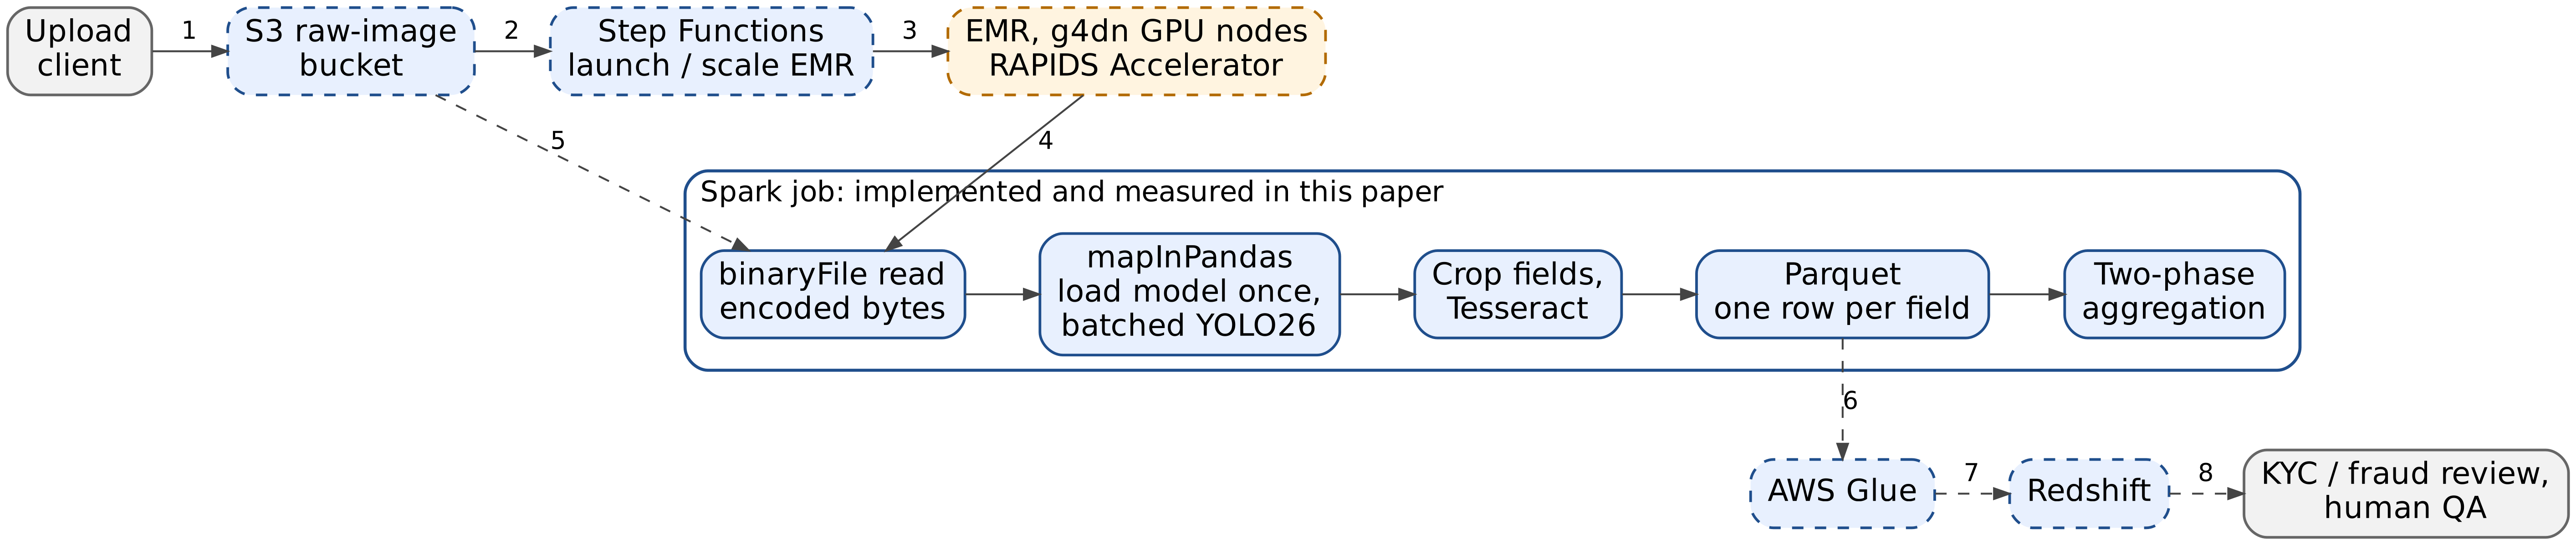
\includegraphics[width=0.98\textwidth]{figures/architecture.png}
\caption{Target architecture. The Spark job (solid) is implemented and measured here on a two-core CPU. Dashed components, including EMR with GPU nodes, Step Functions, Glue, and Redshift, are design only and were not exercised.}
\label{fig:arch}
\end{figure*}

\subsection{Spark job}
The job reads images with Spark\textquotesingle{}s \texttt{binaryFile} source, which returns the encoded file bytes unchanged. A \texttt{mapInPandas} function then runs once per partition. It loads the model once, decodes each Arrow batch of images, makes one batched detector call, crops every detected field from the original image, and runs Tesseract in single-line mode on each crop. Signature regions are detected but not read. Output is long format, one row per detected field, written as Parquet. A final step computes per-class mean confidence with a two-phase aggregation: each partition emits a partial sum and count, and Spark performs the final reduce. That step uses cuDF when RAPIDS is installed and pandas otherwise.

\subsection{Target deployment on AWS}
An upload to S3 raises an event, AWS Step Functions \cite{stepfunctions} launches or resizes an Amazon EMR \cite{emr} cluster, the Spark job runs, and structured output reaches Redshift through Glue. On a GPU cluster the detector would run on the device that Spark assigns to each task, using Spark\textquotesingle{}s custom resource scheduling \cite{spark_resources}, with one GPU per task slot. The pipeline module reads that device index from the task context and sets the corresponding Spark configuration when started with \texttt{--gpu}. We could not exercise this path, because no GPU was available, so it is untested.

\subsection{Where this design applies}
The design targets batch and micro-batch workloads, such as an overnight queue of scanned documents or a stream drained every few minutes. It does not target sub-second per-request latency. A cold EMR cluster adds a start-up cost that we did not measure and that no steady-state throughput figure includes. Interactive use would call for a warm cluster, EMR Serverless, or a plain model server in front of the same detector and OCR code.

\section{Implementation and Verified Defects}\label{sec:impl}
Table~\ref{tab:defects} lists the defects found in the first version of this pipeline. Each row records what was observed when the code was run, not what documentation predicts, except where marked as untested.

\begin{table*}[t]
\centering
\caption{Integration defects found by running the pipeline, and the fix applied in the released code.}
\label{tab:defects}
\small
\begin{tabular}{@{}p{0.2\textwidth}p{0.42\textwidth}p{0.32\textwidth}@{}}
\toprule
Defect & Observed behavior & Fix \\
\midrule
Spark \texttt{image} source fed to an image decoder & Returns decoded pixels, not file bytes. A 640 by 960 image gave 1{,}843{,}200 bytes against a 132{,}098 byte JPEG, and \texttt{imdecode} returned \texttt{None}. & Read with \texttt{binaryFile}, which returned bytes identical to the file. \\
Re-opening a path with \texttt{cv2.imread} & An \texttt{s3://} URI returns \texttt{None}. The path cannot be opened by OpenCV. & Decode the bytes Spark already read; never re-open the path. \\
\texttt{mapInPandas} on Spark 3.5.3 with JDK 21 & Fails in the JVM with \texttt{sun.misc.Unsafe or DirectByteBuffer.<init>(long, int) not available}, including with \texttt{--add-opens} and the Netty reflection flag. & Spark 4.0.1 on JDK 21 ran correctly. Spark 3.5 on JDK 17 is the documented alternative and was not tested. \\
Model constructed inside a row-wise UDF & The model loads once per row. Cost measured in Section~\ref{sec:results}. & Load once per partition inside \texttt{mapInPandas}. \\
Per-image Python loop around the model call & Inference is one image at a time. & One batched call per Arrow batch, with a dynamic-batch ONNX export. \\
Manual resize to 640 by 640 & Distorts non-square pages, and every box then needs mapping back to page coordinates. & Pass the original image. Ultralytics letterboxes internally and returns boxes in original pixels. \\
Hard-coded \texttt{device=0} with two concurrent GPU tasks & Two model copies can land on one device. \textit{Untested, no GPU available.} & Read the device from the task context and schedule one GPU per task. \\
cuDF used to count a substring in one JSON string & Too small an operation to benefit from a GPU, and the key it searched for did not match the output schema. & Per-partition partial sums and counts by class, reduced by Spark. \\
\bottomrule
\end{tabular}
\end{table*}

Listing~\ref{lst:partition} shows the core of the corrected pattern. The complete module, tests, and a one-command reproduction are in the released repository.\footnote{\repourl}

\begin{lstlisting}[language=Python,caption={Partition-level detection and OCR (abridged from \texttt{findoc/pipeline.py}).},label={lst:partition}]
def detect_partition(batches):
  device = _task_device()   # GPU from Spark, else CPU
  model = YOLO(SparkFiles.get(name))  # once
  for batch in batches:     # one Arrow batch
    imgs = [cv2.imdecode(
              np.frombuffer(bytes(raw), np.uint8),
              cv2.IMREAD_COLOR)
            for raw in batch["content"]]
    results = model(imgs, device=device)  # 1 call
    for path, im, res in zip(batch["path"],
                             imgs, results):
      for b in res.boxes:   # original pixels
        x1, y1, x2, y2 = map(int,
                             b.xyxy[0].tolist())
        text = pytesseract.image_to_string(
            gray(im[y1:y2, x1:x2]),
            config="--psm 7").strip()
        rows.append((path, cls(b), ..., text))
    yield pd.DataFrame(rows, columns=COLS)
\end{lstlisting}

\section{Experimental Setup}\label{sec:setup}
\textbf{Data.} A deterministic generator renders account forms at 960 by 640 pixels with five field classes: account number, date, amount, name, and signature. Layout, font, field order, noise, and blur vary per document. Every box and every text string is known exactly. The split is 240 training, 60 validation, and 60 test documents, with disjoint random seeds. The test split holds 300 fields, of which 240 carry text.

\textbf{Model.} YOLO26n fine-tuned from the COCO checkpoint for \valTrainEpochs{} epochs at 640 pixels, batch size 8, AdamW, on CPU, in about \valTrainMinutes{} minutes. We use the nano model because it is the one that trains on this hardware. The paper\textquotesingle{}s design uses the largest model on GPUs, and those results would differ.

\textbf{Hardware and software.} Two virtual CPU cores, 7 GB of memory, no GPU. Python 3.13, Spark 4.0.1, OpenJDK 21, Ultralytics 8.4, ONNX Runtime 1.29, Tesseract 5.3.4.

\textbf{Metrics.} A detection is correct if its class matches and its IoU with an unmatched ground-truth box is at least 0.5. We report precision and recall. End-to-end field accuracy is the share of text fields that are both localized and read with an exact string match after whitespace is removed. The baseline is Tesseract run on the full page. We count a field as captured if its exact string appears anywhere in the page text. That rule is lenient, because the baseline is never required to say which field a string belongs to, so it is an upper bound on what page-level OCR delivers and is not a like-for-like extractor.

\textbf{Inference-pattern timing.} The same fine-tuned model scores \valPatDocs{} test documents on two partitions in three configurations: a row-wise UDF that builds the model on every call, and \texttt{mapInPandas} with Arrow batch sizes 1 and 16. Detection only, no OCR, so the comparison isolates the pattern. Each configuration has one discarded warm-up run and \valPatRepeats{} timed runs.

\textbf{Limits of the design.} There is one training seed, and the test split is 60 documents, so intervals are wide and we report Wilson 95 percent intervals where they matter. The dataset is synthetic, clean, and easy by comparison with scanned documents, so absolute accuracy here says little about real documents.

\section{Results}\label{sec:results}
All numbers in this section are generated from the result files in the repository. The confidence threshold for each variant was chosen on the validation split by detection F1, and each variant was then scored once on the test split.

\subsection{Detection and end-to-end accuracy}
Table~\ref{tab:main} compares three operating points of the same fine-tuned model, which reaches a validation mAP50 of \valMapFifty{} and mAP50-95 of \valMapFiftyNinetyFive{}. Those headline scores say little about deployment behavior. At the default confidence of \valDefConf{}, the exported end-to-end head produced \valDefFields{} boxes for 300 true fields, and precision was only \valDefPrec\%. Of those, \valDefDup{} were duplicates of a field that already had a box, with a mean confidence of \valDefDupConf{} against \valDefTopConf{} for the top box of each field, and \valDefMissed{} fields had no box above the threshold. The NMS-free head is therefore not duplicate-free after a short nano fine-tune.

\begin{table}[t]
\centering
\caption{Test-split results, 60 documents and 300 fields (240 with text). P and R are detection precision and recall at IoU 0.5. OCR is exact match among localized text fields. End-to-end (E2E) is the share of text fields both localized and read exactly, with its Wilson 95\% interval.}
\label{tab:main}
\footnotesize
\setlength{\tabcolsep}{3pt}
\begin{tabular}{@{}lccccc@{}}
\toprule
Variant (conf) & P & R & OCR & E2E & 95\% interval \\
\midrule
NMS-free (\valDefConf, default) & \valDefPrec & \valDefRec & \valDefOcrStage & \valDefEndToEnd & \valDefEndToEndLo{} to \valDefEndToEndHi \\
NMS-free (\valFreeConf, tuned) & \valFreePrec & \valFreeRec & \valFreeOcrStage & \valFreeEndToEnd & \valFreeEndToEndLo{} to \valFreeEndToEndHi \\
Class NMS (\valNmsConf, tuned) & \valNmsPrec & \valNmsRec & \valNmsOcrStage & \valNmsEndToEnd & \valNmsEndToEndLo{} to \valNmsEndToEndHi \\
\bottomrule
\end{tabular}
\end{table}

\begin{figure}[t]
\centering
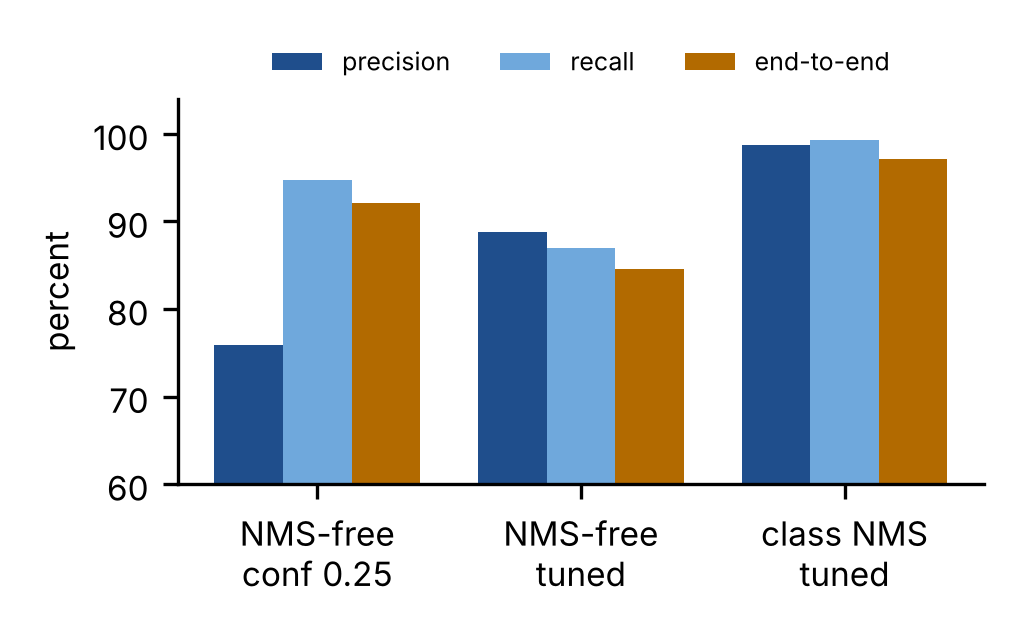
\includegraphics[width=0.95\columnwidth]{figures/variants.png}
\caption{Precision, recall, and end-to-end accuracy for the three operating points in Table~\ref{tab:main}. All values are percentages on one axis.}
\label{fig:variants}
\end{figure}

Three observations follow. First, adding class-wise suppression before OCR lifts precision from \valDefPrec\% to \valNmsPrec\% and end-to-end accuracy to \valNmsEndToEnd\%, and it also removes duplicate crops from the OCR stage. Second, tuning an NMS-free detector for validation F1 chose a high threshold (\valFreeConf{}) that traded away recall, and end-to-end accuracy fell to \valFreeEndToEnd\%, below the untuned default. F1 is not the end-to-end objective, and a threshold chosen for one can hurt the other. Third, the OCR stage is rarely the bottleneck. Among correctly localized text fields it was exact \valNmsOcrStage\% of the time with class NMS, and \valNmsOcrErrAllAccount{} \valNmsOcrErrCount{} errors were on account numbers: \valOcrErrExamples.

Fig.~\ref{fig:perclass} gives the per-class breakdown for the class-NMS variant. Account number is the weakest class, in both recall (\valRecAccountNumber\%) and OCR (\valOcrAccountNumber\%).

\begin{figure}[t]
\centering
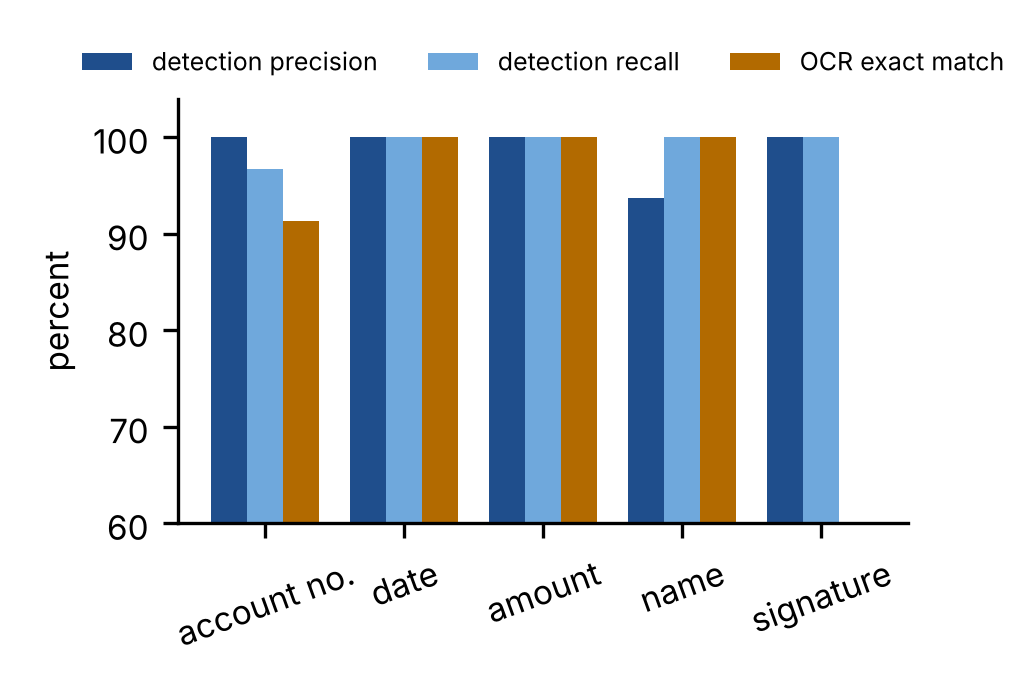
\includegraphics[width=0.95\columnwidth]{figures/per_class.png}
\caption{Per-class detection precision, recall, and OCR exact match for the class-NMS variant on the test split. The vertical axis starts at 60 percent. Signatures are detected but not read.}
\label{fig:perclass}
\end{figure}

\subsection{Comparison with full-page Tesseract}
Full-page Tesseract found \valBaseCapture\% of the 240 text strings somewhere on the page (95\% interval \valBaseLo{} to \valBaseHi), which is higher than the \valNmsEndToEnd\% end-to-end figure. We do not read this as a win for either side. On clean, large, printed text, page-level OCR reads almost every string, and our matching rule is lenient to it, because it never has to say which field a string belongs to. The detect-then-read pipeline pays for field attribution, which the baseline does not provide at all, and on this dataset it does not buy better reading. Whether detection helps on degraded scans, where page-level OCR loses accuracy \cite{thammarak2022,reisswig2019}, is the question this dataset cannot answer. Baseline cost was \valBaseSecPerDoc{} seconds per document on one process.

\subsection{Inference pattern}
Table~\ref{tab:pattern} and Fig.~\ref{fig:pattern} compare three ways of running the same detector over \valPatDocs{} documents in Spark on two partitions, with detection only. All three produced the same \valPatBoxes{} boxes, so they compute the same thing.

\begin{table}[t]
\centering
\caption{Inference pattern timing, mean and standard deviation of \valPatRepeats{} runs after one warm-up. CPU only, two cores.}
\label{tab:pattern}
\small
\begin{tabular}{@{}lccc@{}}
\toprule
Pattern & Seconds & Docs/s & Speedup \\
\midrule
Row-wise UDF, model per row & \valPatRowUdfSec{} $\pm$ \valPatRowUdfSd & \valPatRowUdfDps & 1.0 \\
\texttt{mapInPandas}, batch 1 & \valPatPartOneSec{} $\pm$ \valPatPartOneSd & \valPatPartOneDps & \valPatPartOneSpeedup \\
\texttt{mapInPandas}, batch 16 & \valPatPartSixteenSec{} $\pm$ \valPatPartSixteenSd & \valPatPartSixteenDps & \valPatPartSixteenSpeedup \\
\bottomrule
\end{tabular}
\end{table}

\begin{figure}[t]
\centering
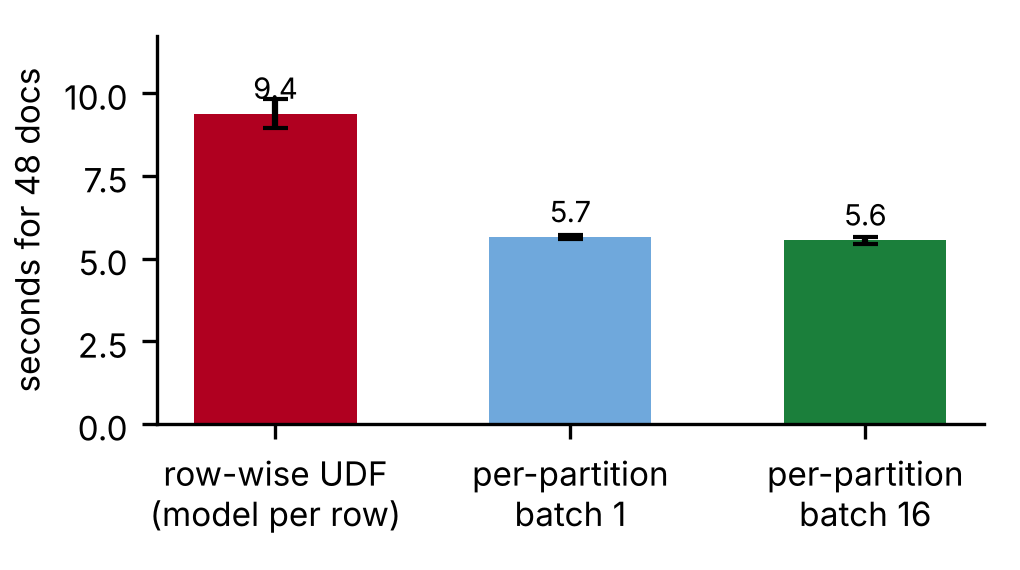
\includegraphics[width=0.95\columnwidth]{figures/pattern.png}
\caption{Wall time for \valPatDocs{} documents under three inference patterns. Error bars are one standard deviation over \valPatRepeats{} runs.}
\label{fig:pattern}
\end{figure}

Loading the model once per partition was \valPatPartSixteenSpeedup{} times faster than loading it per row. The implied cost of one model load is about \valPatLoadMs{} ms, which is small because the nano model is small, and the benefit would grow with a larger model and a CUDA context to initialize, which we did not measure. Arrow batch size 16 was not distinguishable from batch size 1 here (\valPatPartSixteenSec{} against \valPatPartOneSec{} seconds, within one standard deviation). The batching benefit that matters on a GPU is therefore untested by this experiment.

\subsection{Replication on a GPU}\label{sec:gpu}
We repeated the whole protocol once on a single NVIDIA \valGpuName{} GPU in Google Colab, with the same code, settings and Tesseract version. A recorded environment file shows that ONNX Runtime used the \valGpuProvider{} provider and that the \valGpuHashMatches{} test images were produced (SHA-256 prefix \valGpuTestHash), so Table~\ref{tab:gpu} compares the same documents. Training and the confidence sweep were run again, so the weights and the chosen thresholds differ from the CPU run. Spark still ran in local mode with two partitions, so this is a device check and does not exercise Spark GPU scheduling or the RAPIDS Accelerator.

\begin{table}[t]
\centering
\caption{Same protocol on CPU (two cores) and on one \valGpuName{} GPU. Both are single runs on the same 60 test documents.}
\label{tab:gpu}
\small
\begin{tabular}{@{}lcc@{}}
\toprule
 & CPU & \valGpuName{} \\
\midrule
Training time & \valTrainMinutes{} min & \valGpuTrainSeconds{} s \\
Val.\ mAP50 / mAP50-95 & \valMapFifty{} / \valMapFiftyNinetyFive & \valGpuMapFifty{} / \valGpuMapFiftyNinetyFive \\
Class NMS: P / R, \% & \valNmsPrec{} / \valNmsRec & \valGpuNmsPrec{} / \valGpuNmsRec \\
Class NMS: end to end, \% & \valNmsEndToEnd{} & \valGpuNmsEndToEnd{} \\
NMS-free, tuned: end to end, \% & \valFreeEndToEnd{} & \valGpuFreeEndToEnd{} \\
NMS-free, conf 0.25: end to end, \% & \valDefEndToEnd{} & \valGpuDefEndToEnd{} \\
Duplicates at conf 0.25 & \valDefDup{} & \valGpuDefDup{} \\
Row-wise UDF, s & \valPatRowUdfSec{} & \valGpuPatRowUdfSec{} \\
\texttt{mapInPandas}, batch 16, s & \valPatPartSixteenSec{} & \valGpuPatPartSixteenSec{} \\
Speedup, batch 16 & \valPatPartSixteenSpeedup{} & \valGpuPatPartSixteenSpeedup{} \\
\bottomrule
\end{tabular}
\end{table}

Detection and reading replicate: class-wise suppression again removed all duplicates and gave \valGpuNmsEndToEnd\% end-to-end accuracy (95\% interval \valGpuNmsEndToEndLo{} to \valGpuNmsEndToEndHi), and without it the end-to-end head again emitted duplicates (\valGpuDefDup{} at confidence 0.25). The ordering of the three variants is the same on both devices. Differences of a few points between the two columns cannot be separated into device effects and training variance, because each column is one training run on a 60-document test set, and we did not test them for significance. The per-partition speedup over the row-wise pattern held (\valGpuPatPartSixteenSpeedup{} times), but the GPU did not make this job faster. Every pattern was slower on the GPU than on the CPU, for example \valGpuPatPartSixteenSec{} against \valPatPartSixteenSec{} seconds at batch 16. A plausible reason is that a nano model on 640-pixel images is too small to repay device transfers and the initialization of two CUDA contexts, but we did not profile it. Training was the exception, and was much faster on the GPU. The GPU row therefore supports the same conclusions as the CPU run and shows no inference benefit for this small model.

An earlier run on the same GPU is worth recording. It gave only \valFallbackEndToEnd\% end-to-end accuracy because Colab lacked the DejaVu fonts, the generator silently used a different font, and the test images differed. Detection was unaffected (recall \valFallbackNmsRec\%), but reading was not. The released generator now stops with an error in that case. Reading accuracy on synthetic text is sensitive to the rendering environment, which is a further reason to treat all numbers here as properties of this dataset.

\subsection{Dataflow}
Fig.~\ref{fig:dataflow} contrasts the two inference patterns that Table~\ref{tab:pattern} measures.

\begin{figure}[t]
\centering
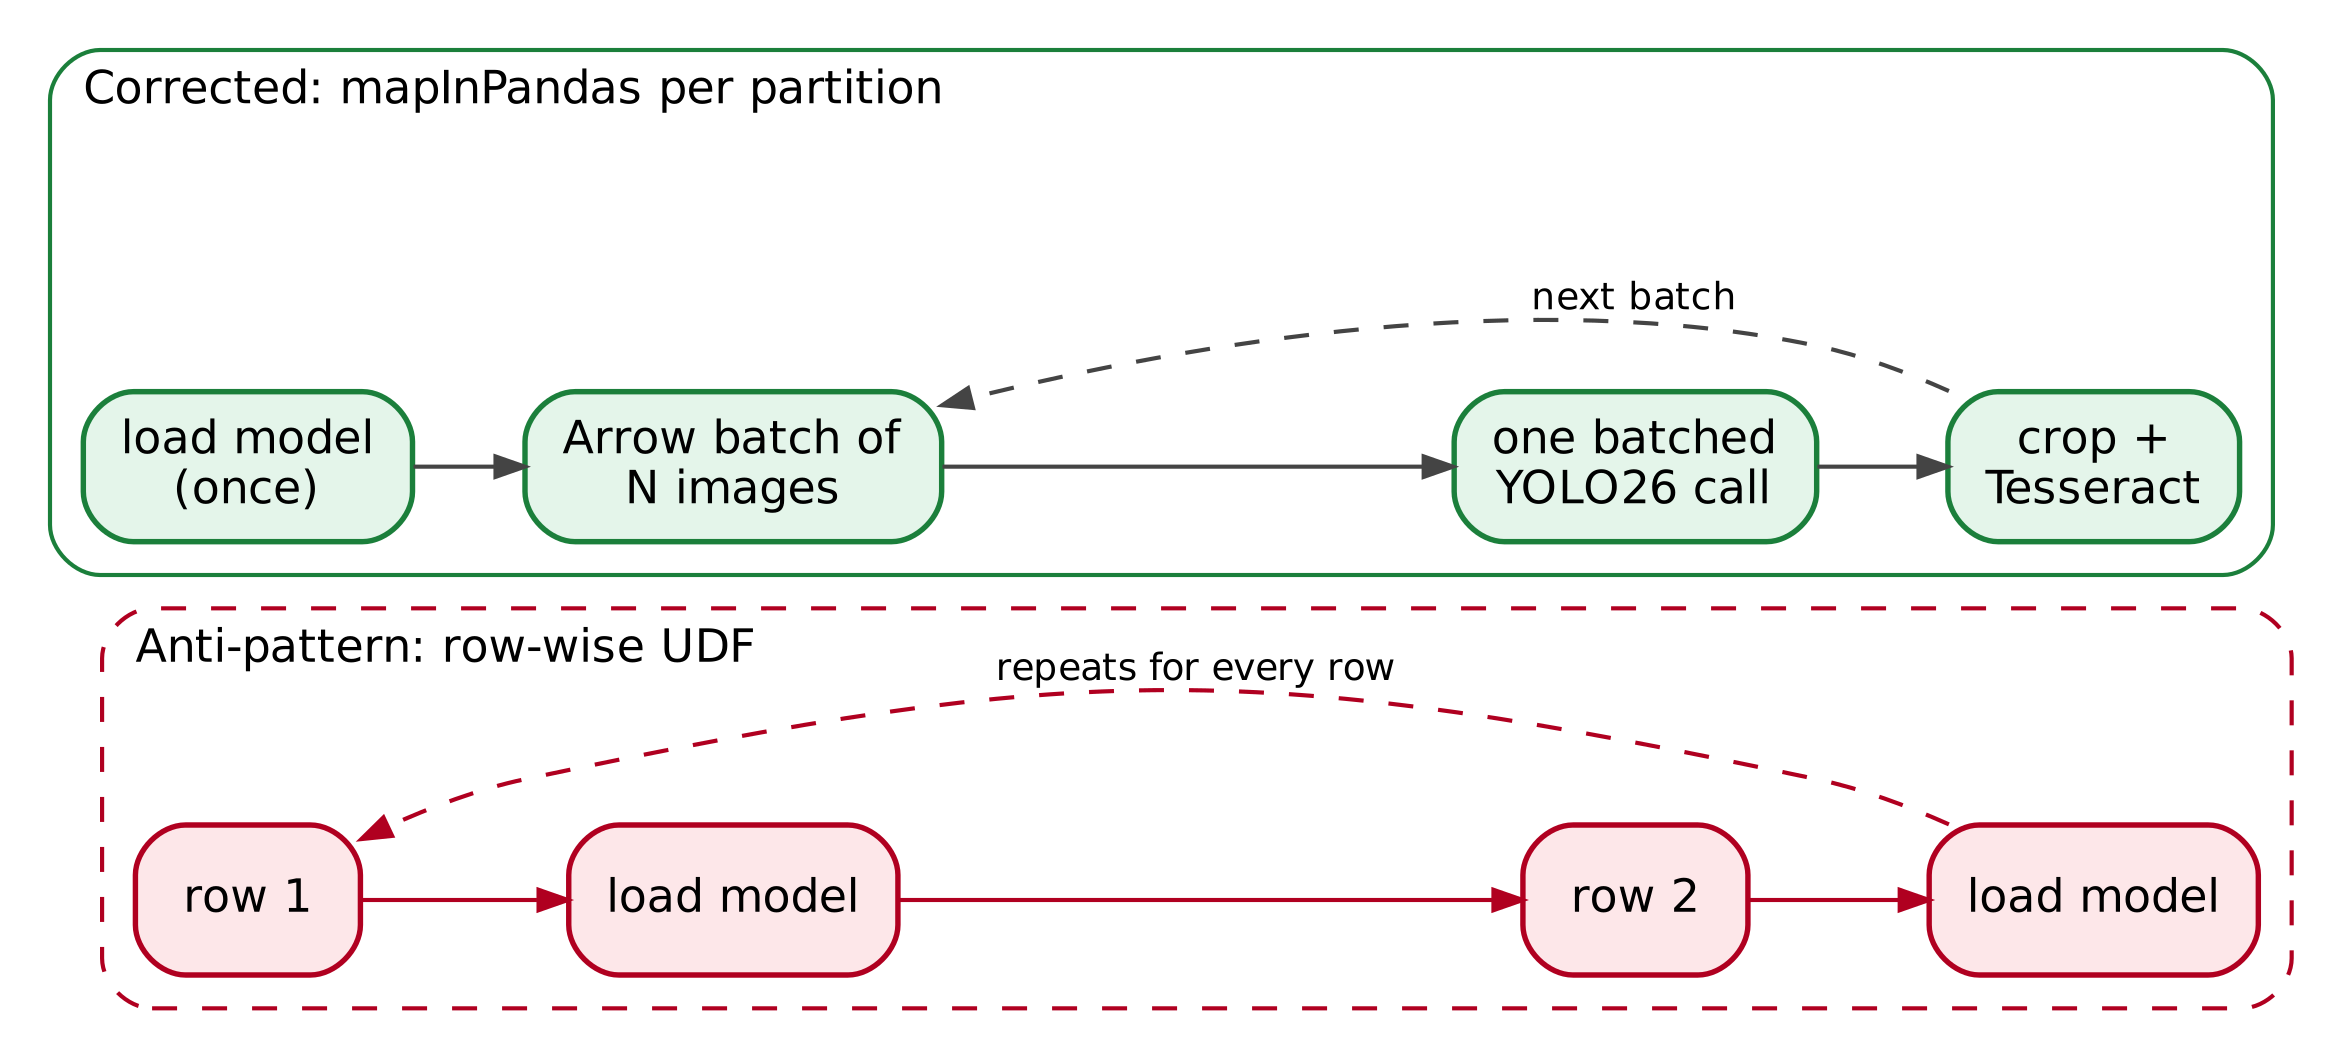
\includegraphics[width=0.95\columnwidth]{figures/dataflow.png}
\caption{Row-wise UDF versus partition-level \texttt{mapInPandas}. The first reloads the model for every row. The second loads it once per partition and then scores Arrow batches.}
\label{fig:dataflow}
\end{figure}

\section{Discussion and Limitations}
\textbf{What this supports.} The pipeline runs end to end under Spark, produces field-labeled text, and is reproducible from one repository. Loading the model per partition is faster than per row, and detection quality at a fixed threshold can differ sharply from the threshold-free mAP that training reports.

\textbf{What it does not support.} The dataset is synthetic, clean, and generated by one randomized form generator with three fonts and varied layout, noise and blur, so it is easy, and the high validation mAP reflects that. The results do not show that detection beats full-page OCR on real documents, and on this data it did not. There is one training run per device and a 60-document test split, so intervals are wide. The detector is the nano model. We ran the protocol on CPU and once on a single GPU in local Spark mode. Multi-node scaling, cluster start-up, cost, Spark GPU scheduling with the RAPIDS Accelerator, and Amazon Textract were not measured, and the cluster GPU configuration in the released code is untested. Stronger baselines, such as LayoutLMv3 \cite{huang2022layoutlmv3}, Donut \cite{kim2022donut}, and other open OCR engines, were not run.

\textbf{Cold start.} The batch design assumes cluster start-up cost is amortized over a queue of documents. It is a poor fit for sub-second interactive requests, for which a warm cluster or a dedicated model server is the better choice.

\textbf{Next steps.} The most informative next experiment is the same protocol on real, degraded scans with field-level labels, where the comparison with page-level OCR could go either way, followed by the GPU path on EMR with a larger model, where device use may matter more than it did here.

\section{Ethical Considerations}
Checks and identification documents contain sensitive personal data. All data here is synthetic. Any use of real documents should follow the institution\textquotesingle{}s data-governance process and data-minimization principles such as those in the GDPR \cite{gdpr}, with encryption at rest, separate access scopes for raw images and structured output, and human review for low-confidence detections rather than automated decisions. Synthetic data from one generator does not establish fair performance across banks, regions, and languages, and that should be tested directly.

\section{Conclusion}
We built and released a Spark pipeline that detects financial form fields with YOLO26 and reads each with Tesseract, and we checked it by running it. The integration defects were real and are cataloged. On clean synthetic forms the pipeline reaches \valNmsEndToEnd\% end-to-end field accuracy with class-wise suppression, the end-to-end head emitted duplicates without it, and full-page OCR read the same strings at least as well, without saying which field each belonged to. Loading the model once per partition was \valPatPartSixteenSpeedup{} times faster than per row on CPU, and \valGpuPatPartSixteenSpeedup{} times on one GPU, where the nano model gained no inference speed. Real scanned documents, cluster-scale GPU execution, and stronger baselines are the open questions, and the released code is meant to make those experiments cheap to run.

\begin{thebibliography}{99}
\bibitem{smith2007} R. Smith, "An overview of the Tesseract OCR engine," in \emph{Proc. Int. Conf. Document Analysis and Recognition (ICDAR)}, vol.~2, 2007, pp.~629 to 633.
\bibitem{thammarak2022} K. Thammarak, P. Kongkla, Y. Sirisathitkul, and S. Intakosum, "Comparative analysis of Tesseract and Google Cloud Vision for Thai vehicle registration certificate," \emph{Int. J. Electrical and Computer Engineering}, vol.~12, no.~2, pp.~1849 to 1858, Apr. 2022.
\bibitem{reisswig2019} C. Reisswig, A. R. Katti, M. Spinaci, and J. H{\"o}hne, "Chargrid-OCR: end-to-end trainable optical character recognition for printed documents using instance segmentation," arXiv:1909.04469, 2019.
\bibitem{textract} Amazon Web Services, "Amazon Textract." [Online]. Available: \url{https://aws.amazon.com/textract/}
\bibitem{redmon2016} J. Redmon, S. Divvala, R. Girshick, and A. Farhadi, "You only look once: unified, real-time object detection," in \emph{Proc. IEEE Conf. Computer Vision and Pattern Recognition (CVPR)}, 2016, pp.~779 to 788.
\bibitem{wang2024yolov9} C.-Y. Wang, I.-H. Yeh, and H.-Y. M. Liao, "YOLOv9: learning what you want to learn using programmable gradient information," in \emph{Proc. European Conf. Computer Vision (ECCV)}, 2024.
\bibitem{wang2024yolov10} A. Wang, H. Chen, L. Liu, K. Chen, Z. Lin, J. Han, and G. Ding, "YOLOv10: real-time end-to-end object detection," in \emph{Advances in Neural Information Processing Systems (NeurIPS)}, 2024.
\bibitem{jocher2026yolo26} G. Jocher, J. Qiu, M. Liu, S. Lyu, F. C. Akyon, and M. E. Kalfaoglu, "Ultralytics YOLO26: unified real-time end-to-end vision models," arXiv:2606.03748, 2026.
\bibitem{zhao2024doclayout} Z. Zhao, H. Kang, B. Wang, and C. He, "DocLayout-YOLO: enhancing document layout analysis through diverse synthetic data and global-to-local adaptive perception," arXiv:2410.12628, 2024.
\bibitem{huang2022layoutlmv3} Y. Huang, T. Lv, L. Cui, Y. Lu, and F. Wei, "LayoutLMv3: pre-training for document AI with unified text and image masking," in \emph{Proc. ACM Int. Conf. Multimedia}, 2022.
\bibitem{kim2022donut} G. Kim \emph{et al.}, "OCR-free document understanding transformer," in \emph{Proc. European Conf. Computer Vision (ECCV)}, 2022.
\bibitem{jaume2019} G. Jaume, H. K. Ekenel, and J.-P. Thiran, "FUNSD: a dataset for form understanding in noisy scanned documents," in \emph{Proc. Int. Conf. Document Analysis and Recognition Workshops (ICDARW)}, 2019.
\bibitem{huang2019sroie} Z. Huang, K. Chen, J. He, X. Bai, D. Karatzas, S. Lu, and C. V. Jawahar, "ICDAR2019 competition on scanned receipt OCR and information extraction," in \emph{Proc. Int. Conf. Document Analysis and Recognition (ICDAR)}, 2019.
\bibitem{zaharia2012} M. Zaharia \emph{et al.}, "Resilient distributed datasets: a fault-tolerant abstraction for in-memory cluster computing," in \emph{Proc. USENIX Symp. Networked Systems Design and Implementation (NSDI)}, 2012, pp.~15 to 28.
\bibitem{nvidia_udf} NVIDIA, "RAPIDS accelerated user-defined functions," RAPIDS Accelerator for Apache Spark documentation. [Online]. Available: \url{https://nvidia.github.io/spark-rapids/docs/additional-functionality/rapids-udfs.html}
\bibitem{nvidia_rapids} NVIDIA, "RAPIDS Accelerator for Apache Spark," GitHub repository. [Online]. Available: \url{https://github.com/NVIDIA/spark-rapids}
\bibitem{spark_mapinpandas} Apache Software Foundation, "pyspark.sql.DataFrame.mapInPandas," Apache Spark documentation. [Online]. Available: \url{https://spark.apache.org/docs/latest/api/python/reference/pyspark.sql/api/pyspark.sql.DataFrame.mapInPandas.html}
\bibitem{spark_resources} Apache Software Foundation, "Custom resource scheduling and configuration overview," Apache Spark configuration documentation. [Online]. Available: \url{https://spark.apache.org/docs/latest/configuration.html}
\bibitem{gdpr} European Parliament and Council of the European Union, "Regulation (EU) 2016/679 (General Data Protection Regulation)," \emph{Official Journal of the European Union}, 2016.
\end{thebibliography}

\end{document}
